\documentclass[a4paper]{jpconf}
\usepackage{graphicx}


\usepackage{slashed}
\usepackage{subfigure}
%\usepackage{rotating}
\usepackage{multirow}
\usepackage{amsmath}
%\usepackage{units}
\setkeys{Gin}{width=\linewidth,totalheight=\textheight,keepaspectratio}
\graphicspath{{fig/}}

%
% My Macros
%
\usepackage{graphicx}
%\usepackage{drftcite}
\usepackage{pstricks}
\usepackage[figuresright]{rotating}
%
%
% Macro declarations
%
%---- SLASH
\def\slasha#1{#1\hskip-0.65em /}  %slasha per caratteri piccoli
\def\slashb#1{#1\hskip-1.3em /}   %slashb per quelli grandi
\def\slashc#1{#1\hskip-.4em /}
%
%---- UNITA` DI MISURA
\def \pb        {{\rm \, pb}}
\def \fb        {{\rm \, fb}}
\def \ipb       {{\rm \, pb^{-1}}}
\def \ifb       {{\rm \, fb^{-1}}}
\def \eV        {{\rm \,  eV}}
\def \keV       {{\rm \, keV}}
\def \MeV       {{\rm \, MeV}}
\def \GeV       {{\rm \, GeV}}
\def \TeV       {{\rm \, TeV}}
\def \TeVc      {\TeV/c}
\def \TeVcc     {\TeV/c^2}
\def \GeVc      {\GeV/c}
\def \GeVcc     {\GeV/c^2}
\def \MeVc      {\MeV/c}
\def \MeVcc     {\MeV/c^2}
%
%---- SIMBOLI
\def\ga{\mathrel{\raise.3ex\hbox{$>$\kern-.75em\lower1ex\hbox{$\sim$}}}}
\def\la{\mathrel{\raise.3ex\hbox{$<$\kern-.75em\lower1ex\hbox{$\sim$}}}}
\newcommand {\lesssim}
     {\,\raisebox{-0.6ex}{$\stackrel{\textstyle<}{\textstyle\sim}$}\,}
\newcommand {\gtrsim}
     {\,\raisebox{-0.6ex}{$\stackrel{\textstyle>}{\textstyle\sim}$}\,}
\newcommand{\ckm}{$\checkmark$}
%
%---- MISCELLANEA
%\newcommand {\slashed}[1] { \mbox{\rlap{\hbox{/}} #1 }}
\newcommand {\onehalf}    {\raisebox{0.1ex}{${\frac{1}{2}}$}}
\newcommand {\fivethirds} {\raisebox{0.1ex}{${\frac{5}{3}}$}}
\newcommand {\OR}         {{\tt OR}\,}
\newcommand {\BR}         {{\rm BR}\,}
\newcommand {\rts}        {\sqrt{s}}
\newcommand {\lumi}       {\mathcal{L}}
\newcommand {\Lumi}       {\int\lumi\mathrm{d}t}
\newcommand {\gradi}    {^\circ}
\newcommand {\de}         {\partial}
\newcommand {\um}         {\, \mu \rm m}
\newcommand {\nm}         {\rm \, nm}
\newcommand {\us}         {\, \mu \rm s}
\newcommand {\cm}         {\rm \, cm}
\newcommand {\mm}         {\rm \, mm}
\newcommand {\m}          {\rm \, m}
\newcommand {\km}         {\rm \, km}
\newcommand {\V}          {\rm \, V}
\newcommand {\T}          {\rm \, T}
\newcommand {\kV}         {\rm \, kV}
\newcommand {\kVm}        {\rm \, kV\! / \! m} 
\newcommand {\MVm}        {\rm \, MV\! / \! m} 
\newcommand {\ns}         {\rm \, ns} 
\newcommand {\ps}         {\rm \, ps} 
%
%---- THEORY groups & AOB
\newcommand {\gws}        {\mathrm{SU(2)_L \otimes U(1)_Y}}
\newcommand {\sul}        {\mathrm{SU(2)_L}}
\newcommand {\suc}        {\mathrm{SU(3)_C}}
\newcommand {\ul}         {\mathrm{U(1)_Y}}
\newcommand {\uem}        {\mathrm{U(1)_{em}}}
\newcommand {\sigmabar}   {\overline{\sigma}}
\newcommand {\gmunu}      {g^{\mu \nu}}
\newcommand {\munu}       {{\mu \nu}}
\newcommand {\obra}       {\langle 0 |}
\newcommand {\oket}       {| 0 \rangle}
%
%---- THEORY lepton fields
\newcommand {\LL}         {L^{\alpha}_{\mathrm L}}
\newcommand {\LLd}        {L^{\dagger \alpha}_{\mathrm L}}
\newcommand {\lL}         {\ell^{\alpha}_{\mathrm L}}
\newcommand {\lLd}        {\ell^{\dagger \alpha}_{\mathrm L}}
\newcommand {\ld}         {\ell^{\dagger \alpha}}
\newcommand {\lb}         {\overline{\ell}^{\alpha}}
\newcommand {\lR}         {\ell^{\alpha}_{\mathrm R}}
\newcommand {\lRd}        {\ell^{\dagger \alpha}_{\mathrm R}}
\newcommand {\nuL}        {\nu^{\alpha}_{\mathrm L}}
\newcommand {\nuLb}       {\overline{\nu}^{\alpha}_{\mathrm L}}
\newcommand {\nub}        {\overline{\nu}^{\alpha}}
\newcommand {\lept}       {\ell^\alpha}
\newcommand {\neut}       {\nu^{\alpha}}
\newcommand {\nuLd}       {\nu^{\dagger \alpha}_{\mathrm L}}
\newcommand {\Phid}       {\Phi^\dagger}
%
%---- THEORY quark fields
\newcommand {\up}         {u^{\alpha}}
\newcommand {\ub}         {\overline{u}^{\alpha}}
\newcommand {\down}       {d^{\alpha}}
\newcommand {\db}         {\overline{d}^{\alpha}}
\newcommand {\QL}         {Q^{\alpha}_{\mathrm L}}
\newcommand {\QLd}        {Q^{\dagger \alpha}_{\mathrm L}}
\newcommand {\UL}         {U^{\alpha}_{\mathrm L}}
\newcommand {\ULd}        {U^{\dagger \alpha}_{\mathrm L}}
\newcommand {\UR}         {U^{\alpha}_{\mathrm R}}
\newcommand {\URd}        {U^{\dagger \alpha}_{\mathrm R}}
\newcommand {\DL}         {D^{\alpha}_{\mathrm L}}
\newcommand {\DLd}        {D^{\dagger \alpha}_{\mathrm L}}
\newcommand {\DR}         {D^{\alpha}_{\mathrm R}}
\newcommand {\DRd}        {D^{\dagger \alpha}_{\mathrm R}}
\newcommand {\bfell}      {\ell\kern-0.4em
                           \ell\kern-0.4em
                           \ell\kern-0.4em
                           \ell }
\newcommand {\obfell}     {\overline{\ell}\kern-0.4em
                           \overline{\ell}\kern-0.4em
                           \overline{\ell}\kern-0.4em
                           \overline{\ell}}
\newcommand {\bfH}      {\, {\cal H}\kern-0.5em \kern-0.4em
                           {\cal H}\kern-0.5em \kern-0.4em
                           {\cal H}\kern0.1em }
\newcommand {\obfH}     {\, \overline{\cal H}\kern-0.5em \kern-0.4em 
                           \overline{\cal H}\kern-0.5em \kern-0.4em 
                           \overline{\cal H}\kern0.1em }
%
%---- PARTICELLE
\def \b             {{\mathrm b}}
\def \t             {{\mathrm t}}
\def \charm         {{\mathrm c}}
\def \d             {{\mathrm d}}
\def \u             {{\mathrm u}}
\def \e             {{\mathrm e}}
\def \q             {{\mathrm q}}
\def \g             {{\mathrm g}}
\def \p             {{\mathrm p}}
\def \s             {{\mathrm s}}
\def \n             {{\mathrm n}}
\def \h             {{\mathrm h}}
\def \l             {\ell} 
\def \f             {{\mathrm f}} 
%\def \f             {{f}} 
\def \A             {{\mathrm A}}
\def \B             {{\mathrm B}}
\def \D             {{\mathrm D}}
\def \K             {{\mathrm K}}
\def \X             {{\mathrm X}}
\def \Y             {{\mathrm Y}}
\def \W             {{\mathrm W}}
\def \H             {{\mathrm H}}
\def \Z             {{\mathrm Z}}
\def \S             {{\mathrm S}}
\def \N             {{\mathrm N}}
\def \L             {{\mathrm L}}
\def \R             {{\mathrm R}}
\def \P             {{\mathrm P}}
\def \G             {{\mathrm G}}
%
%---- Higgs
\newcommand {\ho}         {{\h^0}}
\newcommand {\Ho}         {{\H^0}}
\newcommand {\Ao}         {{\A^0}}
\newcommand {\Hpm}        {{\H^\pm}}
\newcommand {\clsb}       {{\mathrm CL_{\rm s+b}}}
\newcommand {\clb}        {{\mathrm CL_{\rm b}}}
%
%---- SUSY
\newcommand {\dm}         {\Delta m}
\newcommand {\dM}         {\Delta M}
\newcommand {\ldm}        {\mbox{``low $\dm$''}}
\newcommand {\hdm}        {\mbox{``high $\dm$''}}
\newcommand {\nnc}        {{\overline{\mathrm N}_{95}}}
\newcommand {\snc}        {{\overline{\sigma}_{95}}}
\newcommand {\susy}       {{supersymmetry}}
\newcommand {\susyc}      {{supersymmetric}}
\newcommand {\aj}         {\mbox{\sf AJ}}
\newcommand {\ajl}        {\mbox{\sf AJL}}
\newcommand {\llh}        {\mbox{\sf LLH}}
%
%---- SPARTICELLE
\newcommand {\rpc}     {{\rm RPC}}
\newcommand {\rpv}     {{\rm RPV}}
\newcommand {\sfe}     {{\tilde{\f}}}
\newcommand {\sfL}     {{\tilde{\f}_{\mathrm L}}}
\newcommand {\sfR}     {{\tilde{\f}_{\mathrm R}}}
\newcommand {\sfone}   {{\tilde{\f}_{1}}}
\newcommand {\sftwo}   {{\tilde{\f}_{2}}}
\newcommand {\sneu}    {{\tilde{\nu}}}
\newcommand {\wino}    {{\mathrm{\widetilde{W}}}}
\newcommand {\bino}    {{\mathrm{\widetilde{B}}}}
\newcommand {\se}      {{\mathrm{\tilde{e}}}}
\newcommand {\seR}     {{\mathrm{\tilde{e}_{R}}}}
\newcommand {\seL}     {{\mathrm{\tilde{e}_{L}}}}
\newcommand {\st}      {{\mathrm{\tilde{\tau}}}}
\newcommand {\stR}     {{\mathrm{\tilde{\tau}_{R}}}}
\newcommand {\stL}     {{\mathrm{\tilde{\tau}_{L}}}}
\newcommand {\stone}   {{\mathrm{\tilde{\tau}_{1}}}}
\newcommand {\sttwo}   {{\mathrm{\tilde{\tau}_{2}}}}
\newcommand {\sm}      {{\mathrm{\tilde{\mu}}}}
\newcommand {\smR}     {{\mathrm{\tilde{\mu}_{R}}}}
\newcommand {\smL}     {{\mathrm{\tilde{\mu}_{L}}}}
\newcommand {\Sup}     {{\mathrm{\tilde{u}}}}
\newcommand {\suR}     {{\mathrm{\tilde{u}_{R}}}}
\newcommand {\suL}     {{\mathrm{\tilde{u}_{L}}}}
\newcommand {\sdo}     {{\mathrm{\tilde{d}}}}
\newcommand {\sdR}     {{\mathrm{\tilde{d}_{R}}}}
\newcommand {\sdL}     {{\mathrm{\tilde{d}_{L}}}}
\newcommand {\sch}     {{\mathrm{\tilde{c}}}}
\newcommand {\scR}     {{\mathrm{\tilde{c}_{R}}}}
\newcommand {\scL}     {{\mathrm{\tilde{c}_{L}}}}
\newcommand {\sst}     {{\mathrm{\tilde{s}}}}
\newcommand {\ssR}     {{\mathrm{\tilde{s}_{R}}}}
\newcommand {\ssL}     {{\mathrm{\tilde{s}_{L}}}}
\newcommand {\stopR}   {{\tilde{\mathrm{t}}_{R}}}
\newcommand {\stopL}   {{\tilde{\mathrm{t}}_{L}}}
\newcommand {\stopone} {{\tilde{\mathrm{t}}_{1}}}
\newcommand {\stoptwo} {{\mathrm{\tilde{t}_{2}}}}
\newcommand {\sto}     {{\tilde{\mathrm{t}}}}
\newcommand {\SQ}      {{\mathrm{\widetilde{Q}}}}
\newcommand {\STO}     {{\mathrm{\widetilde{T}}}}
\newcommand {\glu}     {{\mathrm{\tilde{g}}}}
\newcommand {\sbotR}   {{\mathrm{\tilde{b}_{R}}}}
\newcommand {\sbotL}   {{\mathrm{\tilde{b}_{L}}}}
\newcommand {\sbotone} {{\mathrm{\tilde{b}_{1}}}}
\newcommand {\sbottwo} {{\mathrm{\tilde{b}_{2}}}}
\newcommand {\sbot}    {{\tilde{\mathrm{b}}}}
\newcommand {\squa}    {{\tilde{\mathrm{q}}}}
\newcommand {\squal}   {{\tilde{\mathrm{q}}_{\rm L}}}
\newcommand {\squar}   {{\tilde{\mathrm{q}}_{\rm R}}}
\newcommand {\sqL}     {{\tilde{\mathrm{q}}_{\rm L}}}
\newcommand {\sqR}     {{\tilde{\mathrm{q}}_{\rm R}}}
\newcommand {\snu}     {{\tilde{\nu}}}
\newcommand {\snue}    {{\tilde{\nu}_{\mathrm e}}}
\newcommand {\snum}    {{\tilde{\nu}_{\mu}}}
\newcommand {\snut}    {{\tilde{\nu}_{\tau}}}
\newcommand {\neu}     {{\chi}}
\newcommand {\chap}    {{\chi^+}}
\newcommand {\cham}    {{\chi^-}}
\newcommand {\chapm}   {{\chi^\pm}}

%
%---- SUSY PARAMETRI
\newcommand {\thstop} {\mathrm{\theta_{\tilde{t}}}}
\newcommand {\thsbot} {\mathrm{\theta_{\tilde{b}}}}
\newcommand {\thsqua} {\mathrm{\theta_{\tilde{q}}}}
\newcommand {\Mcha}{M_{\chi^\pm}}
\newcommand {\Mchi}{M_\chi}
\newcommand {\Msnu}{M_{\tilde{\nu}}}
\newcommand {\tanb}{\tan\beta}
%
%---- ABBREVIAZIONI

%
%---- PROCESSI FISICI
\newcommand {\rb}    {{\rm R_{\b}}}
\newcommand {\qq}    {{\q \overline{\q}}}
\newcommand {\bb}    {{\b \overline{\b}}}
\newcommand {\cc}    {{\charm \overline{\charm}}}
\newcommand {\ff}    {{\f \overline{\f}}}
\newcommand {\el}    {{\e ^+}}
\newcommand {\po}    {{\e ^-}}
\newcommand {\ee}    {{\e ^+ \e ^-}}
\newcommand {\fbody} {{\sto \to \b \chi {\rm f \bar{f}'}}}
\newcommand {\gaga}  {\gamma\gamma}
\newcommand {\ggqq}  {\gamma\gamma \rightarrow \q\overline{\q}}
\newcommand {\ggtt}  {\gamma\gamma \rightarrow \tau^{+}\tau^{-}}
\newcommand {\qqg}   {\q\overline{\q}\gamma}
\newcommand {\ttg}   {\tau^{+}\tau^{-}\gamma}
\newcommand {\wenu}  {{\rm We\nu_\e}}
\newcommand {\gsZ}   {\gamma^\star\mathrm{Z}}
\newcommand {\ggh}   {\gamma\gamma\rightarrow{\mathrm{hadrons}}}
\newcommand {\ZZg}   {\mathrm ZZ^{*}/\gamma^{*}}
\newcommand {\ZZ}    {{\mathrm ZZ}}
%
%---- VARIABILI
\newcommand {\zo}      {{z_0}}
\newcommand {\ip}      {{d_0}}
%\newcommand {\thr}     {{T_{\rm thrust}}}
\newcommand {\thr}     {{{\rm thrust}}}
\newcommand {\athr}    {{\hat{\rm a}_{\rm thrust}}}
\newcommand {\ththr}   {{\theta_{\rm thrust}}}
\newcommand {\acol}    {{\Phi_{\rm acol}}}
\newcommand {\acop}    {{\Phi_{\rm acop}}}
\newcommand {\acopt}   {{\Phi_{\rm acop_T}}}
\newcommand {\thpoint} {\theta_{\rm point}}
\newcommand {\thscat}  {\theta_{\rm scat}}
\newcommand {\etwelve} {E_{12\gradi}}
\newcommand {\ethirty} {E_{30\gradi}}
\newcommand {\eiso}[1] {E^{\, \triangleleft 30\gradi}_{#1}}
\newcommand {\phimiss} {{\phi_{\vec{p}_{\rm miss}}}}
\newcommand {\ewedge}  {E(\phi_{\vec{p}_{\rm miss}}\pm 15\gradi)}
%\newcommand {\ewedge}  {{E_{\rm w}}}
\newcommand {\evis}    {E_{\rm vis}}
\newcommand {\etot}    {E_{\rm vis}}
\newcommand {\emis}    {E_{\rm miss}}
\newcommand {\mvis}    {M_{\rm vis}}
\newcommand {\mtot}    {M_{\rm vis}}
\newcommand {\mmis}    {M_{\rm miss}}
\newcommand {\mhad}    {M^{\rm ex \, \ell_1}_{\rm vis}}
\newcommand {\mhadtwo} {M^{\rm ex \, \ell_1\ell_2}_{\rm vis}}
\newcommand {\ehad}    {E^{\rm NH}_{\rm vis}}
\newcommand {\epho}    {E^{\gamma}_{\rm vis}}
\newcommand {\echa}    {E^{\rm ch}_{\rm vis}}
\newcommand {\nch}     {{N_{\rm ch}}}
\newcommand {\elept}   {E_{\rm lept}}
\newcommand {\elepone} {E_{\ell _1}}
\newcommand {\eleptwo} {E_{\ell _2}}
\newcommand {\pvis}    {{\vec{p}_{\rm vis}}}
\newcommand {\pmis}    {{\vec{p}_{\rm miss}}}
\newcommand {\thmiss}  {{\theta_{\pmis}}}
\newcommand {\pt}      {{p_{\rm t}}}
\newcommand {\ptch}    {{p_{\rm t}^{\rm ch}}}
\newcommand {\pch}    {{p^{\rm ch}}}
\newcommand {\pz}      {{p_z}}
\newcommand {\ptnoNH}  {{p_{\rm t}^{\rm ex \, NH}}}
\newcommand {\puds}    {{P_{\rm uds}}}
%
\newcommand {\pmiss}   {{P\!\!\!\,\!/ }}
\newcommand {\emiss}   {{E\!\!\!\,\!/ }}
%
%
% no more of Christian's random capitalization!
% more of mine
\newcommand{\brchal}{\cal{B}($\PCha \rightarrow \ell\nu\PChi\ $)}
\newcommand{\M}{M_{2}}
\newcommand{\Mp}{M_{2}}
\newcommand{\sigbg}{\sigma_{\mathrm{bg}}}
\newcommand{\ww}   {\mathrm {WW}}
\newcommand{\zz}   {\mathrm Z\gamma^{*}}
\newcommand{\ewnu} {\mathrm{eW}\nu}
\newcommand{\eez}  {\mathrm {eeZ}}
\newcommand{\gagall}{{\gamma\gamma\rightarrow \ell\ell }}
\newcommand{\Pstaup}{{\widetilde{\tau}_{1}}}
\newcommand{\Pstaul}{{\widetilde{\tau}_{L}}}
\newcommand{\Pstaur}{{\widetilde{\tau}_{R}}}
\newcommand{\mzero}{m_{0}}
\newcommand{\msnu}{M_{\tilde{\nu}}}
\newcommand{\mcha}{M_{\chi^{\pm}}}
\newcommand{\mchi}{M_{\chi}}
\newcommand{\mstau}{M_{{\widetilde{\tau}_{1}}}}
\newcommand{\atau}{A_{\tau}}
\newcommand{\chsnu}{\PCha \rightarrow \ell \tilde{\nu}}
\newcommand{\chstau}{\PCha \rightarrow \tilde{\tau}_{1}\nu}
\newcommand{\chlep}{\PCha \rightarrow \ell\nu\chi}
\newcommand{\Tcsq}{\mathrm{TeV}/c^2}
% new for thesis
\newcommand{\nobs}{N_{\mathrm{obs}}}
\newcommand{\nlim}{N_{\mathrm{lim}}}
\newcommand{\Brl}{\cal{B}_{\ell}}
\newcommand{\leff} {\mathcal{L}_{\mathrm{eff}}}
\newcommand{\dedx}{{\mathrm{d}}E/{\mathrm{d}}x}
\newcommand{\chtau}{\PCha \rightarrow \tau\nu\chi}
\newcommand{\ssqtw}{\sin^{2}\theta_{\mathrm W}}
%\newcommand{\PSql}{\tilde{\mathrm q}_L}
%\newcommand{\PSqr}{\tilde{\mathrm q}_R}
%\newcommand{\PSq1}{\tilde{\mathrm q}_1}
%\newcommand{\PSq2}{\tilde{\mathrm q}_2}
%\newcommand{\ww}{{\mathrm WW}}
%\newcommand{\zz}{{\mathrm Z\gamma^{*}}}
%\newcommand{\eez}{{\mathrm eeZ}}
\newcommand{\nnz}{{\mathrm \nu\bar{\nu}Z}}
% added by bill
\def \ggll    {\gamma\gamma \rightarrow \ell^{+}{\ell}^{-}}
\def \tautau  {\mathrm \tau^{+}\tau^{-}}
\def \ffg  {f\bar{f}(\gamma)}
\def \lll   {\ell^{+}{\ell}^{-}}
\def \ww   {\mathrm WW}
\def \zz   {\mathrm Z\gamma^{*}}
\def \znn  {\mathrm Z\nu\nu}
\def \zee  {\mathrm Zee}
\def \rts  {\sqrt{s}}
\def \mstop {m_{\tilde{\mathrm{t}}}}
\def \msnu  {m_{\tilde{\nu}}}
\def \elow   {E_{12^{\circ}}}
\def \gev    { \, \mathrm{GeV}/\it{c}^{\mathrm{2}}}
\def \gvm    { \, \mathrm{GeV}/\it{c}}
\def \mx     {M_{\mathrm{eff}}} 
\newcommand{\neutr}{\chi}
%end fabio



%dalla mia pretesi

%\def \X             {\mathrm X} 
%\def \V             {\mathrm V} 
\def \Zcc           {\Z \to \charm \bar{\charm} }
\def \Zbb           {\Z \to \b \bar{\b} }
\def \decDS         {\D^{*+} \to \D^0 \pi^+}
\def \decsDS        {\D^{*+} \to \D^0 \pi^+_s}
\def \deckp         {\D^{0} \to \K^- \pi^+}
\def \deckppp       {\D^{0} \to \K^- \pi^+ \pi^+ \pi^-}
\def \deckpp        {\D^{0} \to \K^- \pi^+ \pi^0}
\def \deckpS        {\D^{0} \to \K^- \pi^+ (\pi^0)}
\def \decskp        {\D^{*+} \to \pi^{+}_{s} \K^- \pi^+}
\def \decskppp      {\D^{*+} \to \pi^{+}_{s} \K^- \pi^+ \pi^+ \pi^-}
\def \decskpp       {\D^{*+} \to \pi^{+}_{s} \K^- \pi^+ \pi^0}
\def \decskpS       {\D^{*+} \to \pi^{+}_{s} \K^- \pi^+ (\pi^0)}
\def \epsc          {\varepsilon_{\charm}}
\def \epsb          {\varepsilon_{\b}}
\def \pctod         {P_{\charm \to \D^*}}
\def \pbtod         {P_{\b \to \D^*}}
%\def \R             {{\mathrm R}}
\def \Gbb           {\Gamma_{\b\bar{\b}}}
\def \Gcc           {\Gamma_{\charm\bar{\charm}}}
\def \Gh            {\Gamma_{\mathrm h}}
%
% End of my macros
%

\def\centeron#1#2{{\setbox0=\hbox{#1}\setbox1=\hbox{#2}\ifdim
\wd1>\wd0\kern.5\wd1\kern-.5\wd0\fi
\copy0\kern-.5\wd0\kern-.5\wd1\copy1\ifdim\wd0>\wd1
\kern.5\wd0\kern-.5\wd1\fi}}
\def\ltap{\;\centeron{\raise.35ex\hbox{$<$}}{\lower.65ex\hbox{$\sim$}}\;}
\def\gtap{\;\centeron{\raise.35ex\hbox{$>$}}{\lower.65ex\hbox{$\sim$}}\;}
\def\gsim{\mathrel{\gtap}}
\def\lsim{\mathrel{\ltap}}


% Definitions
\def \usedlumi {4.51\fbinv}
\def \chic {\chi_{c}}
\def \Chizero {\chi_{c0}}
\def \Chione {\chi_{c1}}
\def \Chitwo {\chi_{c2}}
\def \theratio {N_{\Chitwo}/N_{\Chione}}
\def \eoneetwo {{\varepsilon_{1}/\varepsilon_{2}}} 
\def \JPsi{\rm J/\psi}
\def \cPgg{\gamma}
\def \pt{$\p_{\rm T}$}

% A useful Journal macro
\def\Journal#1#2#3#4{{#1} {\bf #2}, #3 (#4)}

\begin{document}
\title{An innovative seeding technique for photon conversion reconstruction at CMS}

\author{$^1$D~Giordano and $^2$G~Sguazzoni}

\address{$^1$CERN, Information Technology Department, Experiment Support Group, Geneva, Switzerland}
\address{$^2$INFN, Firenze, Italy}


\ead{domenico.giordano@cern.ch, giacomo.sguazzoni@cern.ch}

\begin{abstract}
The conversion of photons into electron-positron pairs in the detector material is a nuisance in the event reconstruction of high energy physics experiments, since the measurement of the electromagnetic component of interaction products results degraded. Nonetheless this unavoidable detector effect can be also extremely useful. The reconstruction of photon conversions can be used to probe the detector material and to accurately measure soft photons that come from radiative decays in heavy flavor physics. In fact a converted photon can be measured with very high momentum resolution by exploiting the excellent reconstruction of charged tracks of a tracking detector as the one of CMS at LHC. The main issue is that photon conversion tracks are difficult to reconstruct for standard reconstruction algorithms. They are typically soft and very displaced from primary interaction vertex. An innovative seeding technique that exploits the peculiar photon conversion topology, successfully applied in the CMS track reconstruction sequence, is presented. The performances of this technique and the substantial enhancement of photon conversion reconstruction efficiency are discussed. Application examples are given.
\end{abstract}


%\thispagestyle{empty}
\section{Introduction}
\label{introductions}

The precise and efficient determination of charged-particle momenta is a
critical component of the physics program of the LHC~\cite{lhc} experiments, 
as it impacts the ability to
reconstruct leptons, charged hadrons, jets, and photon conversions, which
are the basic physics objects needed to study $pp$ collisions.
Achieving the necessary momentum resolution requires precise tracking in a high magnetic field. This has been obtained by ATLAS~\cite{atlas} and CMS~\cite{cms} -- the two LHC general purpose experiments  --  adopting a design with the inner tracking systems in a solenoidal magnetic field, followed by electromagnetic and hadronic calorimeters, and finally by muon detectors. 

At LHC 
%the inner detectors operates in a hostile environment: 
the large number of tracks in each bunch crossing, which result from several proton-proton interactions, produce many hits in the tracking detectors, making track reconstruction difficult. In order to mitigate this issue the hit occupancy is kept low using highly granular sensors and, consequently, a high number of electronic channels (millions) for their front-end readout at the cost of an increase of material in the tracking volume. These channels need to be powered, controlled, read-out through  complex systems of cables and optical fibers. Moreover they have to dissipate a considerable amount of heat, hence a capillary (permeating??) cooling system is also required.
The consequent amount of material  contained in the detectors and support structures, the associated electronics, and the power-supply and cooling services is not negligible and has effect on the tracking performance because of multiple scattering, energy loss and electron bremsstrahlung. For this reason the reconstruction algorithms have to properly take into account the amount of material in the tracking volume: material that needs to be well measured.  
The material within the tracking volume affects also the overall event topology and its reconstruction, because of photon conversions and nuclear interactions modifying the energy flow through the inner detector.

The unavoidable detector effects due to the tracker material can be also turned into extremely useful tool. For instance the reconstruction of photon conversions can be used to probe the detector material and to accurately measure soft photons produced in radiative decays of heavy flavor particles. In fact a converted photon can be measured with very high momentum resolution by exploiting the excellent reconstruction of charged tracks by the tracking detector. 
 
In this paper we will discuss the impact of the photon conversions and their reconstruction on tracking.  We will refer to the CMS detector, even if most of the concepts discussed can be applied also to other detectors. 
In the following sections a description of the CMS detector will be provided, as well as some examples of the  problems and bonus due to the photon conversions.
We will summarize the current techniques for the reconstruction of photon conversions and describe an innovative technique that allows to increase their reconstruction efficiency.


\section{The CMS detector}



The Compact Muon Solenoid (CMS) features an all-silicon tracker, a lead tungstate crystal electromagnetic calorimeter (ECAL), and a brass-scintillator hadronic calorimeter (HCAL), all contained inside a  $3.8\,{\rm T}$  superconducting solenoid.
The strong magnetic field  enables the measurement of charged
particle momenta over more than four orders of magnitude, from less than
$100\MeVc$ to more than $1\TeVc$, by reconstructing their trajectories as they
traverse the CMS inner tracking system.  
The iron return yoke of the solenoid is interspersed with gas detectors that are used to identify muons.


The CMS Tracker, shown
in~Fig.~\ref{fig:tklayout}, consists of 1\,440 silicon pixel and 15\,148 silicon strip detector modules, covering
the region from $4\cm$ to $110\cm$ in radius, and within $280\cm$ on either
side of the collision point along the LHC beam axis. The tracker
acceptance extends up to a pseudo-rapidity of $\left | \eta \right | < 2.5$.
The pseudo-rapidity $\eta$ is defined as $\rm  -log[tan(\theta/2)]$, where $\theta$ is the polar angle with respect to the direction of the counter-clockwise beam, and $\phi$ is the azimuthal angle.
The tracker detector  provides an impact parameter resolution of $\sim$\,15~$\mu$m and a transverse momentum ($p_{\rm T}$) resolution of about 1.5\,\% for 100~GeV/$c$ particles.
The calorimeter towers are projective and finely segmented, with $\rm \Delta\phi \sim \Delta\eta \sim 0.087$ in the central region, allowing precise reconstruction of the $e/\gamma$ position and energy.  

\begin{figure}[h!]
  \begin{center}
    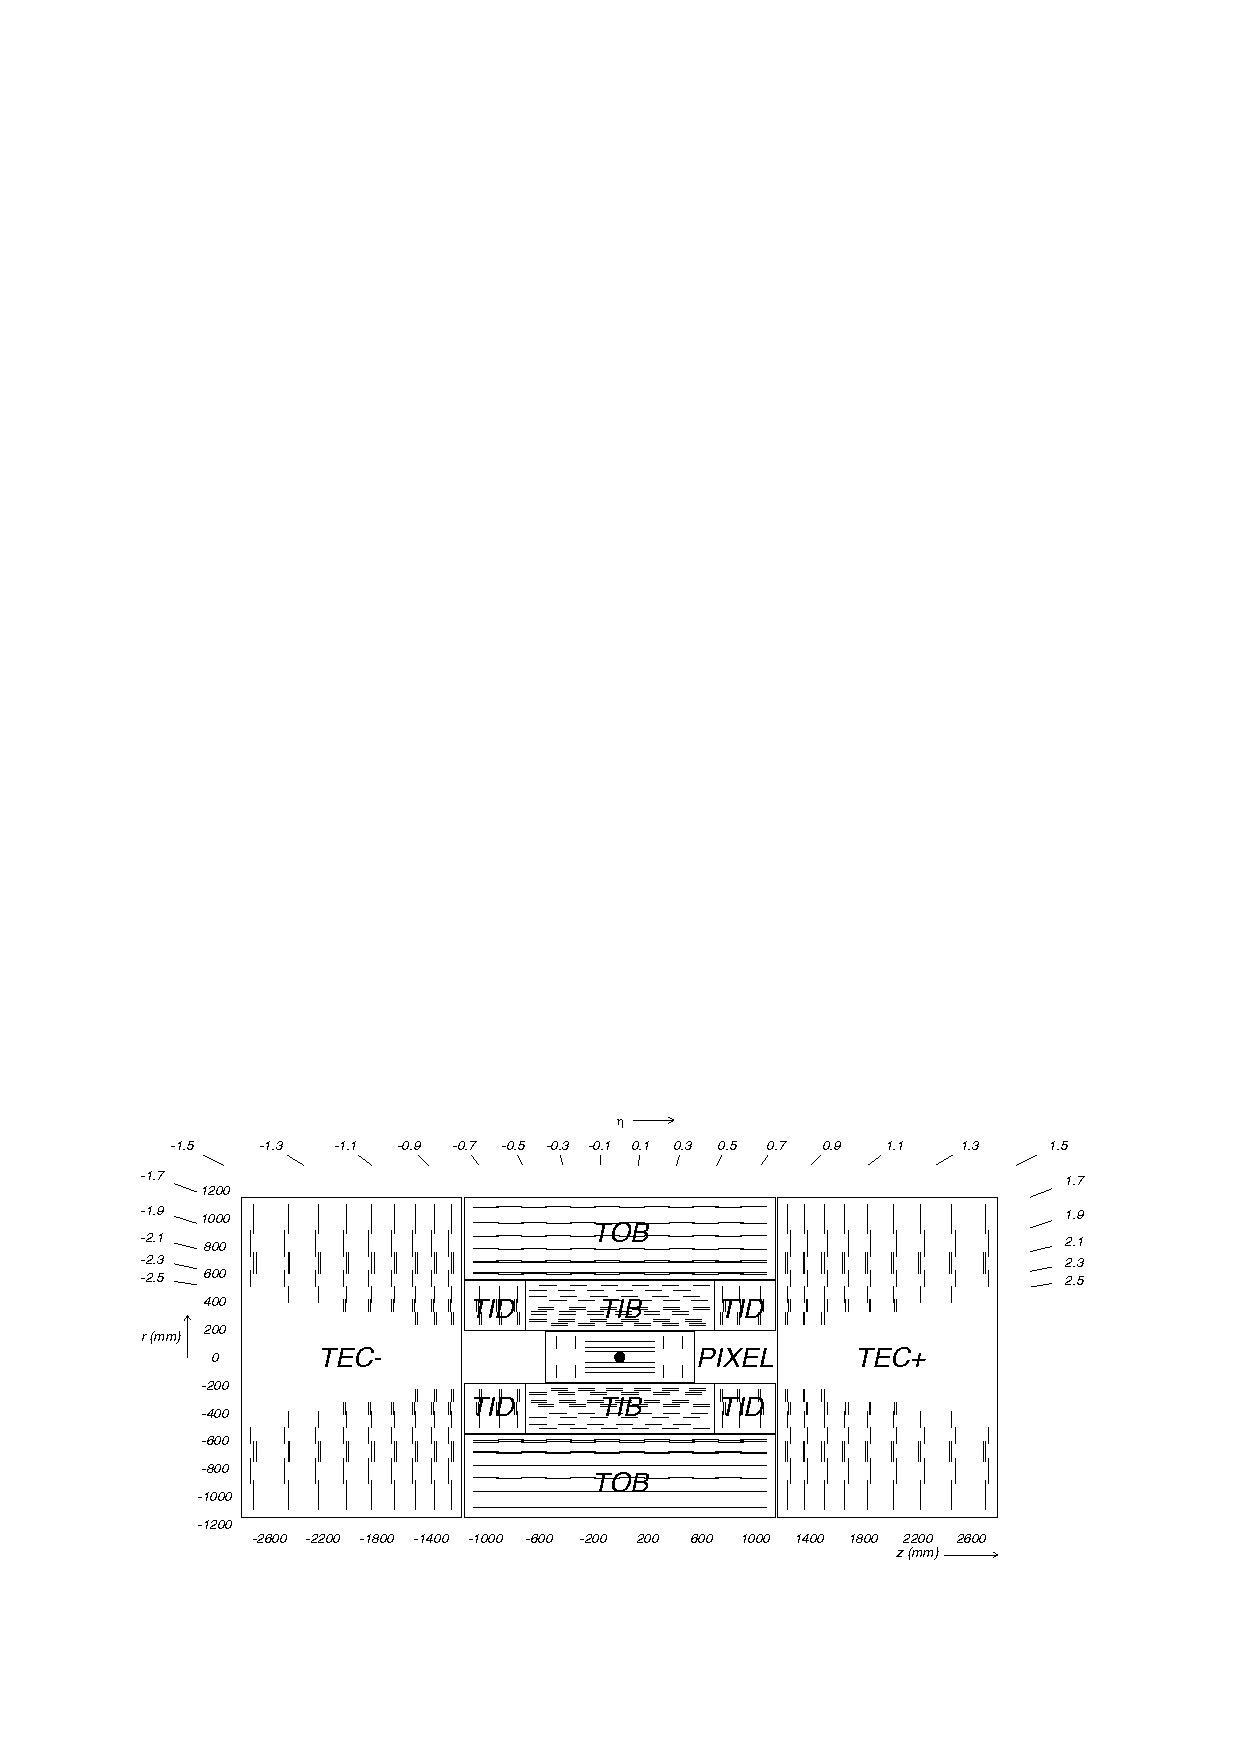
\includegraphics[width=0.8\textwidth]{fig/general_layout.pdf}
    \caption{Schematic cross section through the CMS tracker. Each line represents a detector module. Double lines indicate back-to-back modules which deliver stereo hits.}
    \label{fig:tklayout}
  \end{center}
\end{figure}

\begin{figure}[h!]
  \begin{center}
    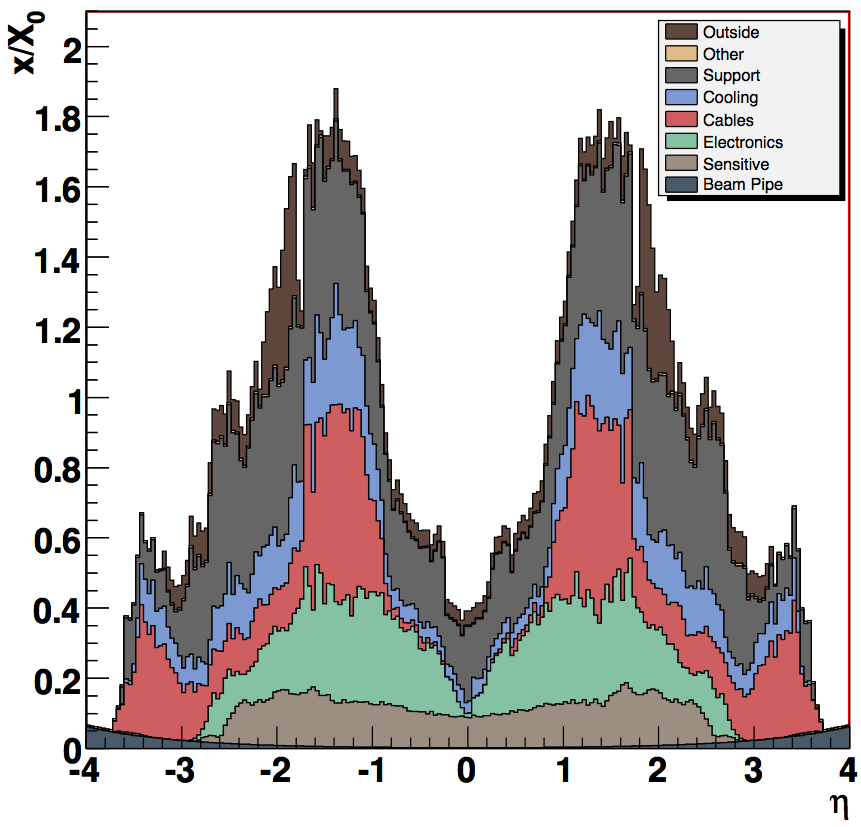
\includegraphics[width=0.4\textwidth]{fig/trackerMaterialbudget.png}
    \caption{Material budget in units of radiation length as a function of pseudorapidity $\eta$ broken down into the functional contributions .}
    \label{fig:tkmaterial}
  \end{center}
\end{figure}



Figure~\ref{fig:tkmaterial} shows the material budget of the CMS tracker in units of radiation length (X0). 
The overall material crossed by a particle traversing the Tracker volume can exceed 1 X0. 
It increases from 0.4~X0 at $\eta \sim 0$ to about 1.8~X0 at $|\eta| \sim 1.4$, beyond which it falls to about 1~X0 at $|\eta| \sim 2.5$.
The largest contribution to the Tracker mass is by far represented by the passive structures for which the uncertainty on their overall amount in the real detector is the largest. A small fractional uncertainty on the description of the material can have a sensible impact on the expected physics performance. 



\section{Impact of the photon conversions - TO BE RENAMED???}


As a consequence  of the amount of material shown in Fig.~\ref{fig:tkmaterial}, up to 70\% of photons traversing the CMS Tracker material converts into  $e^+ e^-$ pairs, resulting in a large fraction of secondary electrons. These electrons are  a non-negligible background to prompt electrons from hadron collisions and must be rejected efficiently in many physics analyses that search for signatures containing prompt electrons.

For this purpose 
CMS has developed several methods  to reduce the electron fake rate by  vetoing electron candidates that match photon conversions. Some methods explicitly identify photon conversions, others use information contained in the electron candidate  such as the hit-pattern to infer from the  number of inner missing hits if the track is prompt or not.

Most of these photons are from ${\rm \pi^0}  \to \gamma\gamma$ decays in jets, or from prompt photons.
Another sources of photons undergoing conversion is the high probability of bremsstrahlung before an electron reaches the electromagnetic calorimeter. 

	
Converted photons inside jets can affect also the jet energy measurement or the jet mis-identification, if not properly reconstructed. 
Let's think to a leading $\pi^0$ inside a jet which immediately decays to two photons. The decay is asymmetric such that one photon carries the majority of the $\pi^0$ energy, and that photon then converts in the tracker material in an asymmetric fashion such that an electron carrying most of the photon energy is produced. This leaves the electron track matching to the rest of the electromagnetic energy deposition, resulting in an electron candidate instead of the genuine jet.

Given the asymmetrical distribution of the energy among the two particles in the $e^+ e^-$ pair, the no-leading track can have a very low \pt that, combined with the vertex displacement, make its 
 reconstruction inefficient.
 The same challenge subsists for the reconstruction of soft-\pt photon conversions ($\rm \lsim 3 GeV$) some of which do not even reach the electromagnetic calorimeter.

Another field is the reconstruction of prompt photon for physics analyses like the higgs to gamma gmama.
For energetic primary photon that converts with both tracks impacting the electromagnetic calorimeter, the effect of the conversions is mitigated by the algorithms used to evaluate the energy deposition that group the energy deposits produced along the azimuthal coordinate, to keep into account the opening of the $e^+e^-$ tracks in the plane transverse to the magnetic field.  
Even if energy of high-\pt converted photons  can be entirely collected by the electromagnetic calorimeter, for many analyses it is essential to be able to reconstruct these objects through the two tracks, to profit of the higher direction resolution of these tracks, in order to well better associate the primary vertex from which the original photon belong.  

Until here we have described the inconvenient effects of the photon conversions. As anticipated this phenomenon can be reverted in favor of specific and cutting-edge applications, such as accurately measuring the material inside the Tracker volume, an aspect that is crucial to have a realistic  material description in the track reconstruction. Or such as the spectroscopy of excited states of heavy flavor particles.  

\subsection{Tracker material budget}
A robust method for the material budget estimation, exploited also by many
past experiments, is based on photon conversions. 
Conversion vertices are reconstructed with a typical radial resolution of $\rm \sigma_r~=~0.2-0.5~cm$ and  angular resolution of  $1~{\rm mrad}$, primarily
as a function of pseudo-rapidity.
The idea is that the
material radiography, provided by the position of reconstructed photon
conversion vertices, allows for the visualisation of detector layers
and service structures and that the conversions rate provides an estimate of the amount of material in the
detector volume in terms of radiation lengths.
In Fig.~\ref{fig:convXY} the position of conversion vertices reconstructed in data is shown in the $(x,y)$ plane:
in Fig.~\ref{subfig:convXY_a} the structure at the very centre is the Pixel detector,
surrounded by the shell and rails supporting the Pixel detector, four layers of the Inner Tracker and the first layer of the Outer Tracker.
When restricting the $(x,y)$ view to $\pm 12\cm$, Fig.~\ref{subfig:convXY_c}, the beam pipe is clearly visible, off-centered with respect to
the Pixel detector. 
The  $(z, R)$  view of conversion vertices reconstructed in data is  shown in Fig.~\ref{fig:convRZ};  the less populated
areas  around $|\eta|\sim1.2$ corresponds to transition regions between the Tracker
barrel and endcap sub-components where the larger amount of passive material and the change in the active material topology makes more difficult the reconstruction of displaced vertexes. 
The dedicated seeding described in Sec.~\ref{sec:newSeedingStep} provides a reasonable increase of efficiency, as it will be shown later.

\begin{figure}[h!]
  \begin{center}
   \subfigure[]{
   \label{subfig:convXY_a}
    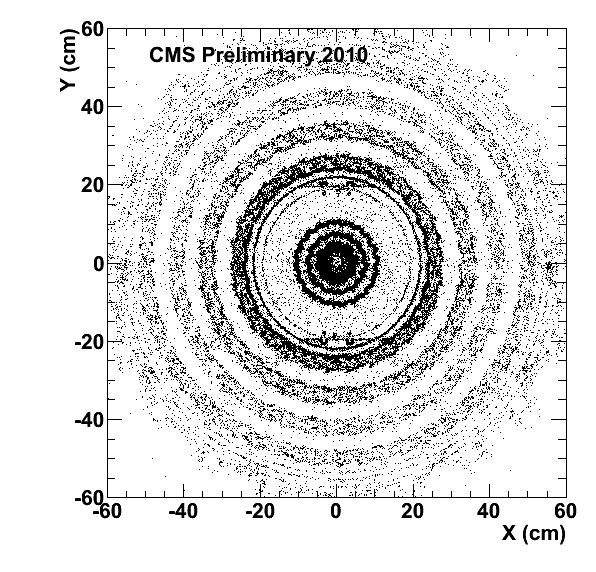
\includegraphics[width=0.40\textwidth]{fig/conversions/ptCut/data_xy.png}}
   \subfigure[]{
   \label{subfig:convXY_c}
    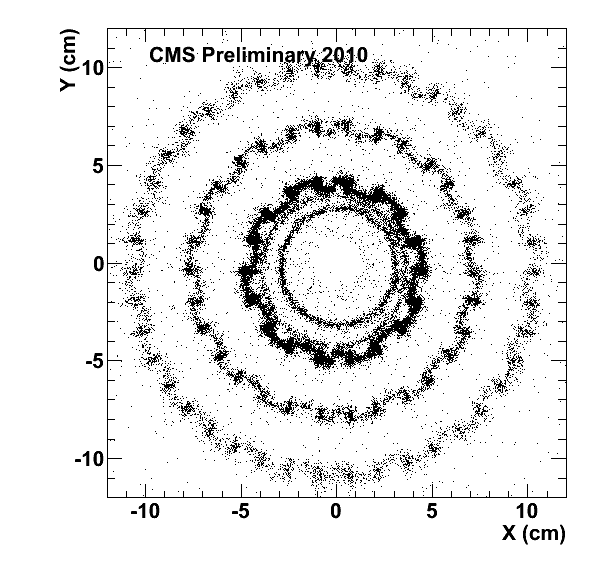
\includegraphics[width=0.40\textwidth]{fig/conversions/ptCut/data_xy_pixel_eta.png}}
    \caption{Conversion vertices in data in the $(x,y)$ plane for $|z|<26\cm$; zoom increases from (a) to (b). 
    Results were obtained on a sample corresponding to 1/nb of integrated luminosity where about 260 000 photon conversions were reconstructed. 

}
    \label{fig:convXY}
  \end{center}
\end{figure}

\begin{figure}[h!]
  \begin{center}
     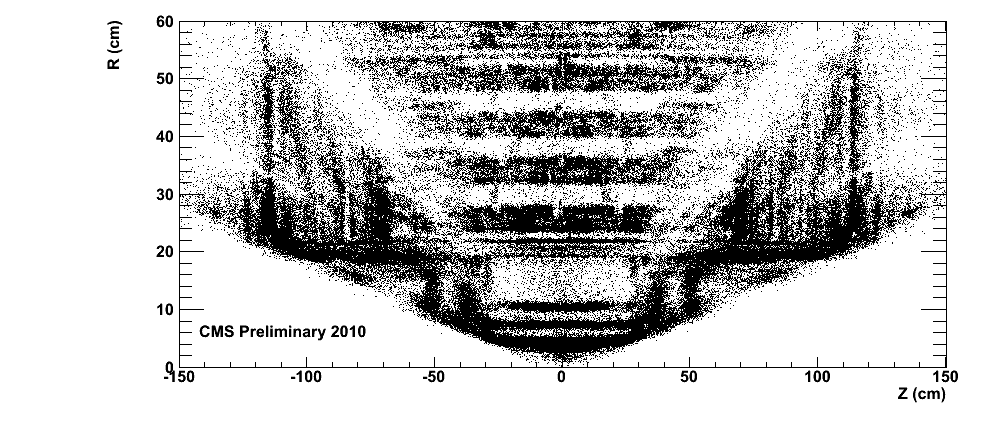
\includegraphics[width=15cm,height=5.5cm]{fig/conversions/ptCut/data_rz.png}
      \caption{Conversion vertices in data the $(z,R)$ plane.}
    \label{fig:convRZ}
  \end{center}
\end{figure}




\begin{figure}[!hbtp]
\centering
%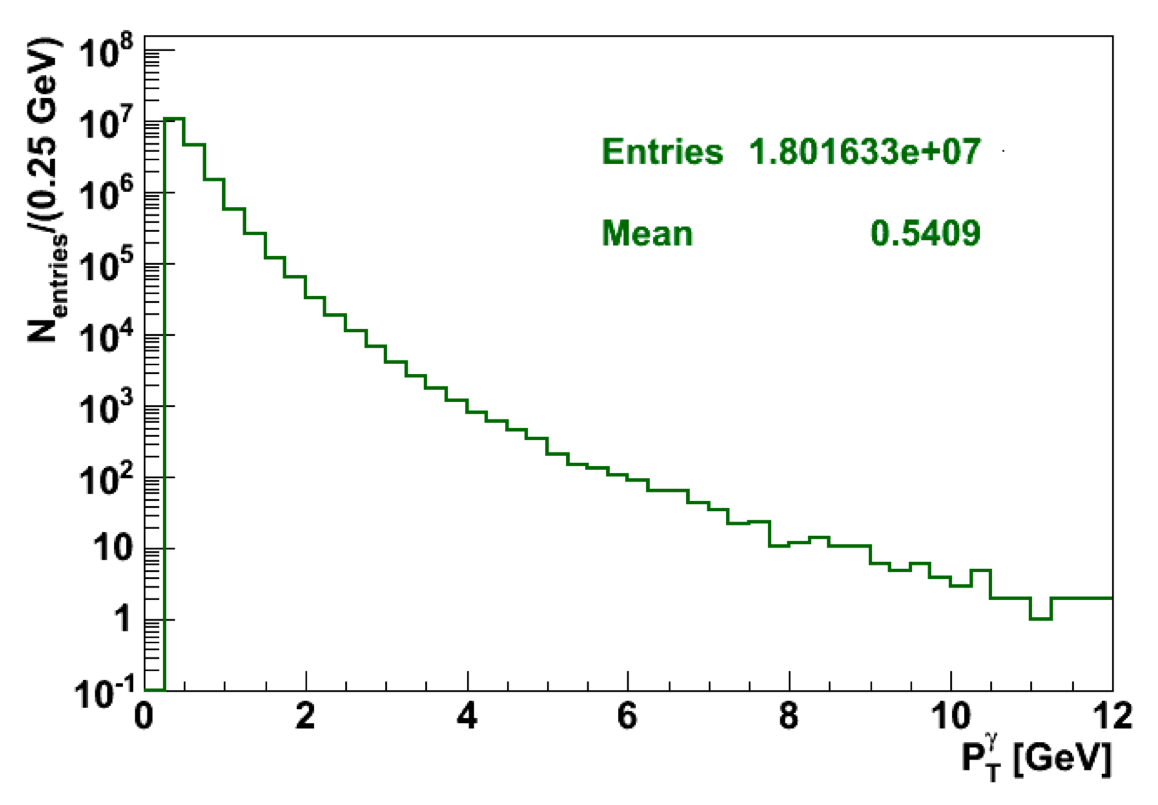
\includegraphics[width=.45\textwidth]{ptMC.png}
\caption{Transverse momentum spectrum of converted photons in minimum
  bias MC events at $\sqrt{s}=900\GeV$.}
\label{ptMC}
\end{figure}



\subsection{Radiative decay of heavy flavor particles}

The measurement is based on the 
reconstruction of the radiative decays to $\JPsi$ plus photon, with the
(relatively low energetic) photons being detected through their 
conversion in electron-positron pairs. 

We select $\Chione$ and $\Chitwo$ candidates by searching for their radiative
decays into the $\JPsi + \cPgg$ final state, with the $\JPsi$ decaying
into two muons. 
Given the small difference between the $\JPsi$ mass, $3096.916\pm0.011\MeVcc$, and the $\Chione$ and $\Chitwo$ masses, $3510.66\pm0.07\MeVcc$ and $3556.20\pm0.09\MeVcc$ respecively~\cite{PDG}, an accurate reconstruction of the photon  
is then needed to finalize the reconstruction of the $\chic$ with
sufficient resolution. In the center of mass of the charmonium states, the photon has an energy of
390\MeV when emitted by the $\Chione$ and of 430\MeV when emitted by the
$\Chitwo$, which results in a $p_T$ of the photon to be measured mostly
between 0.5 and 6\GeVc in the laboratory frame. 


\begin{figure}[t]
    \centering
    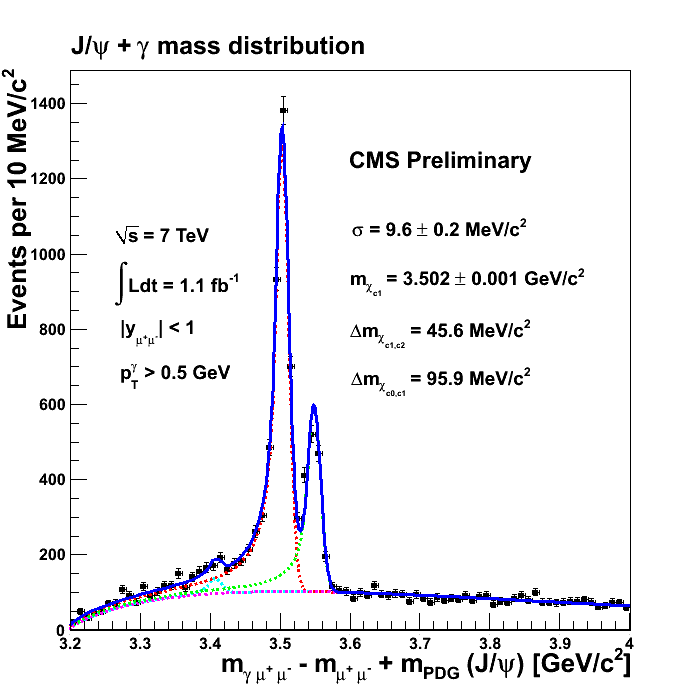
\includegraphics[width=0.6\textwidth]{fig/Chic1fb.png}
    \caption{Invariant mass spectrum for $\chi_c$ candidates with $p_T^{\JPsi}$ between 7.0 and 25.0\GeVc.}
    \label{fig:chic}
\end{figure} 


\begin{figure}[t]
    \centering
    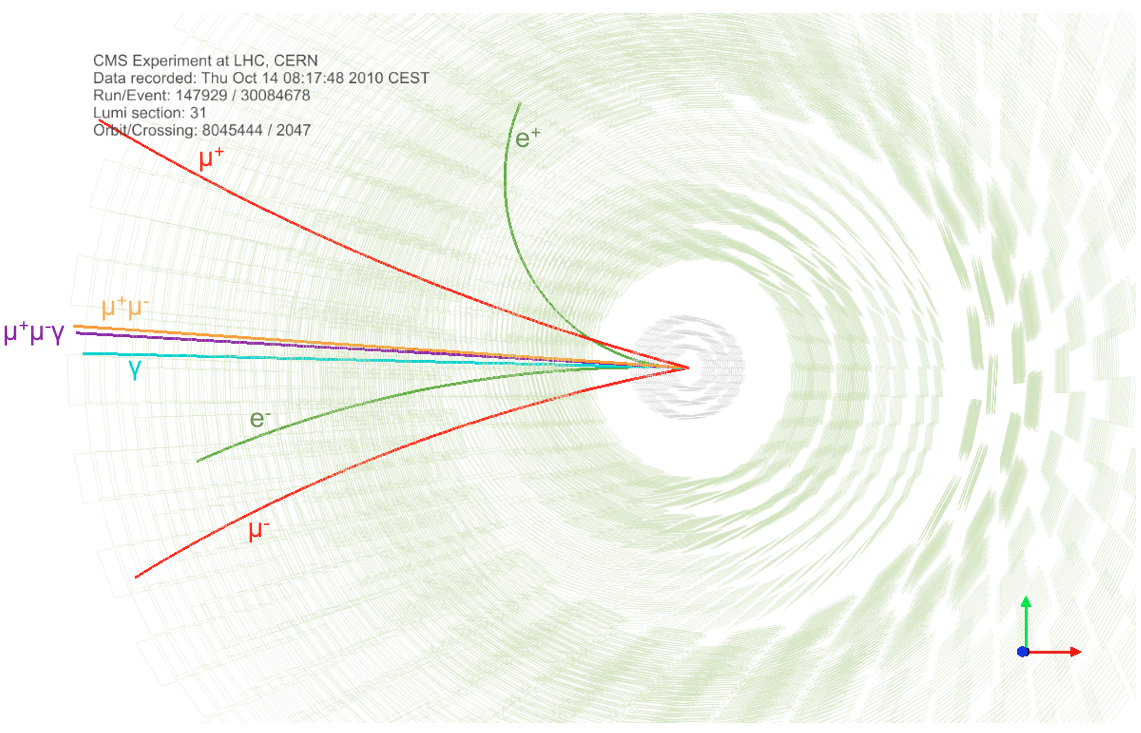
\includegraphics[width=0.6\textwidth]{fig/EvtDisplay.png}
    \caption{Event Display}
    \label{fig:evtdisplay}
\end{figure} 




At such low energies (rarely above 
2.5\GeV in the laboratory), the calorimetric
measurements do not have precisions comparable to those obtainable
when the photon energy is measured through the tracking of the 
electron-positron pair originating from a conversion of the photon, in
the beam pipe or in the inner layers of the silicon tracker. 
Furthermore, the calorimeter (``particle flow") photons do not have 
an accurate assignment of the interaction vertex where they come from,
contrary to the converted photons; this vertexing capability is useful to 
reject combinations of $\Upsilon$ dimuons produced in one pp collision 
with photons produced in another (something especially important in the
presence of a large number of pileup collisions). 


to disentangle the two states, whose masses differ by only
45\MeV.

 On the contrary, a measurement of the momentum of the
electron-positron pair originating from a conversion of the photon, in
the beam pipe or in the inner layers of the Tracker, results in a very
accurate measurement of the photon energy. 

\section{difficulties}

 The drawback 
is the reduced yield, caused by the the low efficiency of their reconstruction as pairs of low momentum tracks displaced with respect to the beam axis.




\section{Photon Conversion Reconstruction}
\label{standard}


Reconstruction of converted photons is hence a crucial step in CMS, and dedicated algorithms have been developed, which make use either of a seeding step which starts from calorimetric cluster [? ] or pairing standard reconstructed tracks [? ].


We use only tracker driven conversion reconstruction since we are dealing with low pT photons (�3 GeV/c) and some of them does not even reach the electromagnetic calorimeter; in this transverse momentum region ECAL seeded conversion reconstruction has a very low reconstruction efficiency, being optimized to reconstruct conversion in a region of pT > 10 GeV/c.



The approach is to select a collection of tracks in which to find conversion candidates, apply the vertex fit to all 24	pairs of tracks passing a preselection, make the final selection of conversion candidates, then veto any matching 25	electron candidates



%CMS AN -2009/173
The collection of tracks used to construct the conversion candidates should provide an inclusive sample covering 36	the widest possible range of conversion position and kinematics. It should also facilitate unambiguous matching 37	to the reconstructed electron candidates.
38	The standard CMS track reconstruction produces an inclusive collection of pixel and tracker-seeded tracks re- 39	sulting from an iterative procedure to include increasingly displaced and/or low pT tracks. These tracks are fit 40	using the standard Combinatorial Kalman Filter (CKF) fitter, which is mathematically equivalent to a global least- 41	squares minimization [2]. This �generalTracks� collection is the most inclusive available from the reconstruction, 42	in particular for lower pT tracks which do not reach the ECal.
43	In addition, there are two ECal-seeded track collections produced as part of the standard conversion reconstruction 44	sequence in CMSSW employing respectively inside-out and outside-in seeding as described in [3]. These collec- 45	tions include very displaced tracks which would not be present in the generalTracks collection, but exclude tracks 46	which have insufficient pT to reach the ECal.
47	Electron candidates use tracks reconstructed with a Gaussian Sum Filter (GSF) fit, which employs a weighted 48	sum of Gaussian components to model the non-Gaussian energy loss distribution for electrons passing through 49	the material. These tracks are either seeded directly from pixel hits matched to the ECal, or refit from existing 50	standard tracks. These tracks are stored in the dedicated �electronGsfTracks� collection. Matching the conversion 51	candidates to the electron candidates is therefore simplest and most efficient if the collection of tracks used to 52	reconstruct conversions includes these GSF tracks. The final collection of tracks used to produce the conversion 53	candidates is created by merging the above four track collections. First the generalTracks plus the two ECal-seeded 54	track collections are merged using the standard algorithm, which removes duplicate tracks by hit sharing. Track 55	quality is used to decide which should take precedence, keeping the track with the larger number of hits, or with 56	the smaller normalized ?2 in the case of an equal number of hits.
57	In order to ensure that all of the electron GSF tracks are included in the final collection, the GSF tracks are merged 58	with the above combined collection again using hit sharing to remove duplicates, but always forcing the GSF track 59	to take precedence. Removing duplicates at the track level ensures that there is no double counting of conversion 60	candidates, although this is not a strict requirement for the conversion removal use case.



Taking the merged track collection as input, a preselection is applied to all opposite-sign pairs of tracks, using an 72	analytic helix intersection and requiring that the point of closest approach has r > 0.9 cm, where r = ??x2 + y2 73	in the absolute coordinate system of the detector.

At the LHC many photons are produced from $\pi^0$ decays in minimum bias events; 
as shown in Figure~\ref{ptMC}, the $p_T$ spectrum of such photons is
very soft and the electron and positron produced in the conversion 
do not have enough transverse momentum to reach the CMS electromagnetic calorimeter.
Therefore, conversions need to be reconstructed with a tracker standalone algorithm.


Standard reconstruction of tracks in
the CMS Tracker is seeded by the hits in the
detector~\cite{TRK-10-001}.  


The detection of photon conversions  relies
on the reconstruction of displaced secondary vertices, and the track
reconstruction algorithm described in~\cite{TRK-10-001} has been tuned
to allow reconstruction of tracks originated into the tracking volume,
as far as at a radius of $60\cm$.


In the Minimum Bias events  photons, mainly coming from
$\pi^0$ decays, are expected to have a very soft spectrum. The electron pairs from conversions are very unlikely to
reach the Electromagnetic Calorimeter (ECAL) and the ECAL cluster-driven track and seed finding method~\cite{NOTE2006005, EGM-10-005}
cannot be applied. The development of the iterative tracking described in~\cite{TRK-10-001}
largely extended the capability of reconstructing low-\pt tracks and displaced vertices.
Furthermore, for the work presented in this Analysis Summary, additional seeding steps were introduced as described in Sec.~\ref{sec:newSeedingSteps}
and exploited here to improve the identification of conversions at large radii.
The tracker-only conversion reconstruction was already partially commissioned with limited statistics
during the LHC runs at $\sqrt{s}=900\GeV$ data~\cite{TRK-10-001}.


Photon conversions are characterized by a pair of
oppositely charged secondary tracks, originating from the photon vertex with an
invariant mass consistent with zero,  which are therefore parallel
to each other at production vertex. The electron-positron pair, then,
opens only in the transverse plane because of the solenoidal magnetic field.


Two methods are used in CMS, ECAL-seeded conversion method and combined conversion method. One method only uses the conversion ECAL-seeded tracks and the 	other takes into account conversion track pairs reconstructed from a combination of standard 	tracks, Gaussian sum filter (Gsf) tracks and conversion ECAL-seeded tracks. 

Both methods (ECAL-seeded and combined) 	fit two oppositely charged tracks to a common vertex with the constraint that the two tracks 	are parallel at the vertex, in both the transverse and longitudinal planes. The methods differ 	mainly in the preselection of the track pairs.

%\subsection{Selection and results}                                                                                                                                                                



In this analysis we use the tracker-driven conversion reconstruction,
already described in~\cite{TRK-10-001}, in~\cite{trk10001} and in~\cite{TRK-10-003}. We
summarize the method here. The algorithm relies on the capability of iterative tracking,
discussed in~\cite{TRK-10-001}, to efficiently reconstruct low-\pt and
displaced tracks, as the ones coming from a photon conversion.

Opposite-sign track pairs are firstly required to satisfy basic
quality criteria, i.e. have more than four hits and a normalised
$\chi^2$ less than 10. Then
the tracker-only conversion finding exploits the conversion pair
signature to distinguish genuine pairs from fake pairs.
Tracks are required to have positive charge-signed transverse impact
parameter (the primary vertex lies outside the track trajectory helix)
and the distance of minimum approach in the $xy$ plane, $d_m$, between $-0.25\cm$
and $1\cm$ where $d_m$ is
%defined as $d_{O_1-O_2} - (R_1 - R_2)$ where
%$d_{O_1-O_2}$ is the distance between the centres of the two track
%circles in the transverse plane and $R_1$ and $R_2$ are the two
%circles radii.
the distance between the two points of tangent approach in the
transverse plane for the helices of the two tracks.



Surviving track pairs are then fitted by a 3D-constrained kinematic vertex 
fitter that imposes the
tracks to be parallel in both the transverse and longitudinal planes.
The pair is retained if the fit converges and its $\chi^2$ probability
is greater than $5\times10^{-4}$ (value used in the $\chi_{c2} / \chi_{c1}$ 
cross-section ratio analysis~\cite{bib:AN-11-332}).
%


\section{Tracking Improvement}
\label{sec:newSeedingStep}


Prompt photons in the event undergoes asymmetric conversion in the tracker material producing one electron carrying the majority of the photon energy. The second electron from the conversion has too low momentum, or the conversion vertex is not reconstructed well, and as a result these events are not found by the conversion finding algorithm and will be identified as a prompt electron.

Hard bremstrahlung photon: There are cases where a lepton undergoes hard bremstrahlung in the tracker material producing a photon with large momentum. This photon undergoes conversion again in subsequent layers of the tracker material in the same way described for the prompt photon category.

photon then converts in the tracker material in an asymmetric fashion such that an electron carrying most of the photon energy is produced. This leaves the electron track matching to the rest of the electromagnetic energy deposition with a reasonable energy over momentum fraction,



The tracks of the resulting electrons from a conversion decay are parallel to each other at the decay point, and re- main so in the r?z plane. This is a unique feature that is the basis of the algorithm we use. To exploit this geometry, all Combinatorial Track Fitter (CTF) tracks within a cone of �R < 0.3 around the electron�s GSF track and with
charge opposite that of the GSF track, are pre-selected. For each of fined


The standard CMS tracking is made of six iterative steps, numbered
from 0 to 5, designed to obtain high efficiency and low fake rate for
tracks coming either from the primary vertex or from displaced decay
vertices while maintaining the overall computing time within the
requirements of CMS offline reconstruction centre.
Because of this constraint, the standard implementation is not optimal
to reconstruct with high efficiency tracks from photon conversions
 since the cuts applied in the standard
reconstruction are too tight for these processes. In fact, those
tracks have usually very low momentum and, especially for displaced
vertices at large radii, they do not point  back to the primary
vertex; therefore, they could be reconstructed only with very relaxed
cuts that would result into unacceptably large computing time during
the pattern recognition.

For the purpose of the present study, an additional dedicated
tracking step is added to the track reconstruction sequence.


 is seeded from pairs of hits
in the Pixel barrel and/or in the Strip Tracker Inner barrel
detectors; 

in the Strip Tracker barrel detectors and/or in the Strip Tracker Inner disks.

The seed trajectories are required
%to originate from a region of radius $25\cm$ and longitudinal half length of $0.5\cm$ and are required                                                                                            
to have a minimum transverse momentum of $0.1$ and $0.2\GeVc$ for the
step 6 and 7, respectively. 

To limit  the large number of seeds is
reduced by selecting topologies compatible with a photon conversion
pair: the total charge has to be zero,



Seeds are then
propagated outward, adding compatible hits and updating the trajectory
until either the detector boundary is reached, or no additional
compatible hits can be found.  In the final stage, the collection of
hits is fit to obtain the best estimate of the track parameters.


 
 
The pattern recognition is then performed allowing for at most one
lost hit and requiring at least three hits. Finally the standard track
fit provides the best estimate of the track parameters.

The impact of the additional step to the reconstruction of conversion
and nuclear interaction vertices can be seen on Fig.~\ref{fig:matItTk}
showing the contribution of the different steps to the vertices
reconstruction, as estimated by the simulation.
The additional step increases by more than a factor two the number of conversions
outside the Pixel detector region and contributes significantly to nuclear
interaction vertices at all radii; step 6 mainly helps finding
conversions in the second and third Pixel detector layers.


\begin{figure}[!hbtp]
\centering
\subfigure[]{
\label{subfig:convItTk}
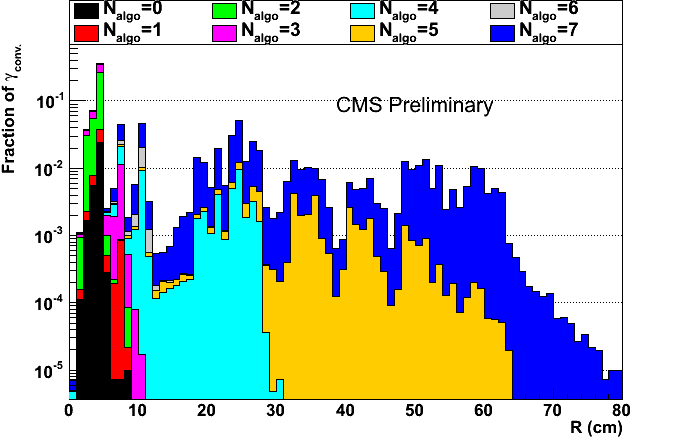
\includegraphics[width=.7\textwidth]{fig/r_algo_BasicCutsJuly12.png}}
\subfigure[]{
\label{subfig:nuclItTk}
\includegraphics[width=.7\textwidth]{fig/r_algo_2010-06-04_NI.png}}
\caption{Fraction of reconstructed vertices as a function of the radius of the vertex
for conversions~\subref{subfig:convItTk} and nuclear
interactions~\subref{subfig:nuclItTk}, for  $|\eta|<1.4$, as estimated
from simulation. The different colors correspond to the largest
iterative step needed to reconstruct the tracks at the vertex.}
\label{fig:matItTk}
\end{figure}

\section{otherseed}

\section{Conclusions}
\label{section_conclusions}


The method here presented provides ...

\section*{References}

\begin{thebibliography}{99}


\bibitem{cms}{CMS Collaboration}.
\newblock {The CMS experiment at the CERN LHC}.
\Journal{\em JINST}{0803}{S08004}{2008}.

\bibitem{steve} S.~Wasserbaech, {\em Computeraized tomography of the
    ALEPH detector}, ALEPH Internal Note, {\tt ALEPH 97-08} (1997);
\bibitem{nancy} N.~Marinelli et al, {\em Photon conversion algorithm},
  CMS Analysis note in preparation;
\bibitem{integrals} H.B.~Dwight, {\em Tables of Integrals and Other
    Mathematical Data}, New York and London, The Macmillan Company (1957);\\
  M.~Abramowitz, I.A.~Stegun, {\em Handbook of Mathematical
  Functions with Formulas, Graphs, and Mathematical Tables}, New York,
  Dover Publications (1972), ISBN 978-0-486-61272-0;
%\emph{}


\bibitem{CMS_NOTE_2006_041}
W.~Adam, B.~Mangano, Th. Speer, and T.~Todorov.
\newblock {Track Reconstruction in the CMS Tracker}.
\Journal {\em CMS Note}{2006/041}{}{2006}.


\bibitem{CMS_PAS_TRK_10_001}
{CMS Collaboration}
\newblock{Tracking and Vertexing Results from First Collisions}.
\\
\newblock{http://cms-physics.web.cern.ch/cms-physics/public/TRK-10-001-pas.pdf}
\\
\Journal{\em CMS Physics Analysis Summary}{TRK-10-001}{}{2010}


\end{thebibliography}
\end{document}
